\section{Numerical solution to the pendulum problem}
In this section, we present and analyze the numerical solution of the filtering problem associated to the pendulum experiment. We then run the SIS and SMC algorithms to approximate the expected value of the full posterior distribution and analyze their empirical convergence properties. As a reference, we also present the result of the MCMC approximation to the complete data set.

In the first experiment, we estimate the solution to the Bayesian inverse problem found by considering all the available data collected during the physical experiment. We use the MCMC algorithm for $10,000$ steps after a burn-in period of $500$ steps and construct the Markov chain using Metropolis-Hasting kernel with Gaussian proposals of variance $0.1$. The burn-in period runs the Markov Chain for $500$ steps without collecting the generated samples needed to reach the region of high probability. After $5$ runs of the algorithm, we find an mean estimate of $\expec{u|y} = 9.86 \pm \mathcal{O}(10^{-3})$ and a variance of $\mathcal{O}(10^{-6})$. This result is consistent with the unnormalized likelihoods presented in Figure \ref{uncertainty-posteriors}, and validate the theoretical results stated in Lemma \ref{sampling-bound}. A typical run of the algorithm is given in Figure \ref{mcmc-figure}.

\begin{figure}[!b]
  \label{mcmc-figure}
  \begin{minipage}{.43\textwidth}
    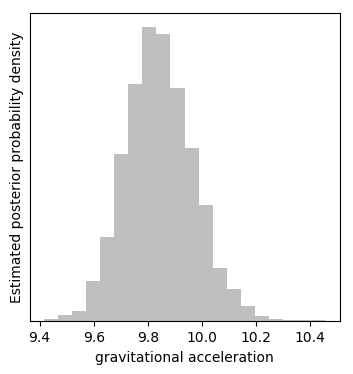
\includegraphics[width=\linewidth]{mcmc}
  \end{minipage}
  \begin{minipage}{.5\textwidth}
    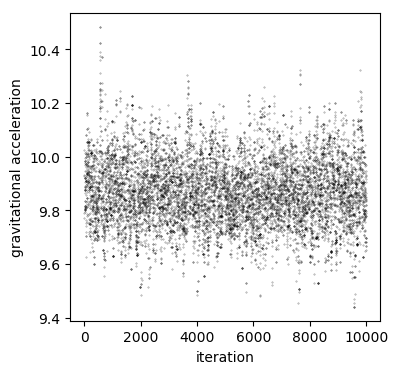
\includegraphics[width=0.97\linewidth]{mcmc-mixin}
  \end{minipage}
  \caption{Left: estimated posterior distribution using $M=10,000$ samples from the MCMC algorithm with burn-in period of $500$ samples. Right: samples of the Markov chain for one run on the MCMC algorithm. We see that the burn-in period allows to have all samples in the zone of high density and converge.}
\end{figure}

\begin{figure}[htbp]
  \begin{minipage}{.5\textwidth}
    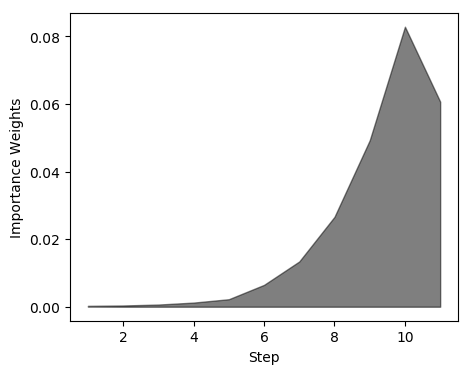
\includegraphics[width=\linewidth]{importance-weights-sis}
  \end{minipage}
  \begin{minipage}{.5\textwidth}
    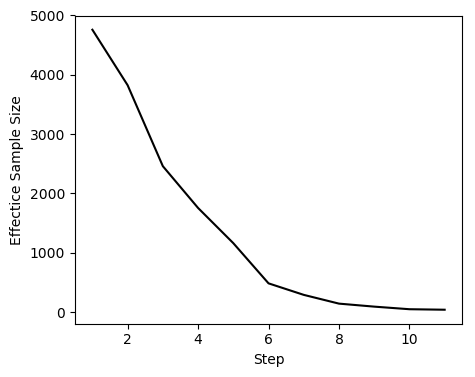
\includegraphics[width=0.97\linewidth]{ess-decay}
  \end{minipage}
  \caption{Left: the evolution of the importance weights of the particle estimates. The upper and lower bounds of the shaded area represent the value of the largest and smaller importance weight of the population. We can see that close to the end, a single particle contain almost all mass of the estimated probability measure. Right: evolution of the ESS over time, we see that after half the total number of iterations, the ESS is already only almost 1.}\label{sis-figure}

  \bigskip
  
  \begin{minipage}{.5\textwidth}
    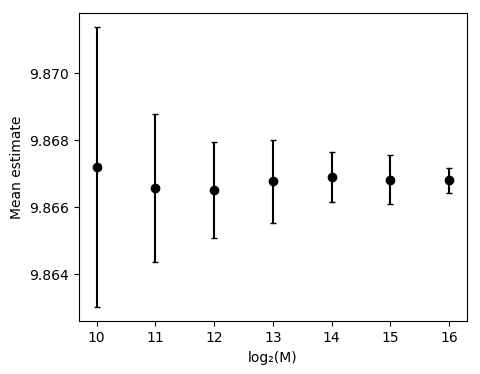
\includegraphics[width=\linewidth]{mean-estimate}
  \end{minipage}
  \begin{minipage}{.5\textwidth}
    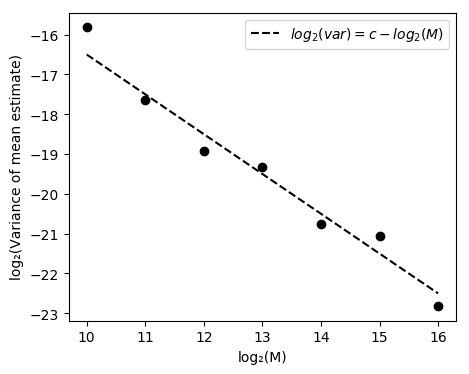
\includegraphics[width=0.97\linewidth]{var-of-estimate}
  \end{minipage}
  \caption{Both plots consider $40$ runs of $M$-particles SMC estimates of the posterior expected value. Left: Each point is the mean and variance over the $40$ SMC runs for each $M$. Right: Logarithmic plot of the variance of $40$ estimates. Line illustrates the asymptotical $\mathcal{O}(M^{-1})$ behaviour of the variance proved in Theorem \ref{smc-convergence}. }\label{smc-figure}
\end{figure}


However, we are interested in approximating the sequence of filtering posterior distributions arising from the pendulum problem where the data only becomes available one observation at a time. In the following experiments, we use the sequence of importance weights given in (\ref{pendulum-weights}). Since we fulfill all assumptions stated in Lemma \ref{easy-lemma}, it also satisfies Assumption \ref{kappa-assumption} and the solution provided by the SIS and SMC algorithms weakly converge in $M$ to the true posteriors. In both algorithms, we use Metropolis-Hastings kernels with Gaussian proposals of variance $0.05$. 

In the second experiment, we illustrate why the step of resampling is crucial in the SMC algorithm. We run the SIS algorithm with $M=5,000$ particles and monitor the ESS as well as the importance weights over time. As expected, the experiment shows that the variance of the weights increases with both very large and very small weights, meaning that most of the probability mass of the particle estimate is contained in only a few estimate. Monitoring the ESS confirms this is also shown by the convergence of the ESS to $1$. This makes the variance These two results are shown in Figure \ref{sis-figure}.

In a last experiment, we run the SMC algorithm with $M_{thresh} = M/2$ for several values of $M$ and repeat the experiment $40$ times per configuration. We use $5$ MCMC updates for the correction step to improve the approximations, this claim is theoretically justified by \cite{marion2018finite}. Figure \ref{smc-figure} reports the result of the experiment, showing the convergence of the posterior expected value estimate.

To conclude this section, we compare computational costs of the MCMC and SMC algorithms. Each time new data becomes available, the MCMC algorithm needs to sequentially re-sample $M$ values from the associated Markov chain. This in turn leads to $M$ evaluations of the likelihood function, requiring to numerically solve $M$ initial value problems. While the SMC algorithm also needs to perform $M$ evaluations of the likelihood function to update the particles, since each particle is independent these evaluations do not need to be made sequentially. This allows to parallelize the evaluation of the likelihood function and potentially strongly reduce the cost of updating an existing estimate as shown by \cite{lee2010utility}.

%%% Local Variables:
%%% mode: latex
%%% TeX-master: "Thesis"
%%% End:
